Let us start with some thermodynamics. Every material has an equation of state.
The equilibrium thermodynamic state of any material can
be constrained if any two state variables are specified.
Examples of state variables include
the pressure $p$ and specific volume $\nu = 1/\rho$, as well as the temperature $T$.

After linearisation, the density depends on temperature and pressure as follows:
\[
\rho(T,p) = \rho_0 \left((1 - \alpha(T-T_0) + \beta_T P \right)
\]
where $\alpha$ is the coefficient of thermal expansion, also called 
thermal expansivity: \index{thermal expansion}
\[
\alpha=-\frac{1}{\rho}\left( \frac{\partial \rho}{\partial T} \right)_p
\]
$\alpha$ is the percentage increase in volume of a material per degree of temperature increase; the
subscript $p$ means that the pressure is held fixed.

$\beta_T$ is the isothermal compressibility of the fluid, which is given by \index{compressibility}
\[
\beta_T = \frac{1}{K} = \frac{1}{\rho}\left( \frac{\partial \rho}{\partial P} \right)_T
\]
with $K$ the bulk modulus. \index{bulk modulus}
%aspect manual
Values of $\beta_T=10^{-12}-10^{-11}$ Pa$^{-1}$ are reasonable for Earth's mantle, with values decreasing by about a
factor of 5 between the shallow lithosphere and core-mantle boundary.
This is the percentage increase in density per unit change in pressure at constant temperature.
Both the coefficient of thermal expansion and the isothermal compressibility can be obtained
from the equation of state.

The full set of equations we wish to solve is given by

\begin{eqnarray}
-\nabla \cdot \left[2\eta \dot{\bm \epsilon}^d({\bm v}) \right] + \nabla p &=& \rho {\bm g} \quad\quad \textrm{in $\Omega$}  \label{eq:stokes-1} \\
\nabla \cdot {\bm v} + \frac{1}{\rho} {\bm v} \cdot {\bm \nabla}\rho&=&0 \quad\quad  \textrm{in $\Omega$}   \label{eq:stokes-2} \\
\rho C_p \left(\frac{\partial T}{\partial t} + \bm v\cdot\nabla T\right) - \nabla\cdot k\nabla T   &=& 
  \rho H  +  2\eta \dot{\bm \epsilon}^d : \dot{\bm \epsilon}^d    +\alpha T \left( \bm v \cdot \nabla p \right) 
\quad\quad   \textrm{in $\Omega$},
  \label{eq:temperature}
\end{eqnarray}

Note that this presupposes that the density is not zero anywhere in the domain.

We use a mixed formulation and therefore  
keep both velocity and pressure as unknowns. We end up having to solve 
the following system:
\[
\left(
\begin{array}{cc}
\K & \G+\W \\ \G^T+\Z & 0 
\end{array}
\right)
\cdot
\left(
\begin{array}{c}
{\cal V} \\ {\cal P}
\end{array}
\right)
=
\left(
\begin{array}{c}
 f \\ h
\end{array}
\right)
\quad\quad
{\rm or,}
\quad\quad
\A \cdot X = rhs
\]
Where $\K$ is the stiffness matrix, $\G$ is the discrete gradient operator, 
$\G^T$ is the discrete divergence operator, ${\cal V}$ the velocity vector, 
${\cal P}$ the pressure vector.
Note that the term $\Z{\cal V}$ derives from term ${\bm v} \cdot {\bm \nabla} \rho$ in the continuity equation. 

Each block $\K$, $\G$ , $\Z$ and vectors $f$ and $h$ are built separately 
in the code and assembled into 
the matrix $\A$ and vector $rhs$ afterwards. $\A$ and $rhs$ are then passed to the solver. 
We will see later that there are alternatives to solve this approach which do not require to 
build the full Stokes matrix $\A$. 

{\sl Remark 1}: the terms $\Z {\cal V}$ and $\W {\cal P}$ are 
often put in the rhs (i.e. added to $h$) so that 
the matrix $\A$ retains the same structure as in the incompressible case. This is indeed 
how it is implemented in ASPECT, see also appendix A of \cite{lezh08}. This however requires more work since the rhs depends 
on the solution and some form of iterations is needed. 

{\sl Remark 2}: Very often the adiabatic heating term  
$\alpha T \left( \bm v \cdot \nabla p \right)$ is simplified as follows:
%aspect manual
If you assume the vertical component of the gradient of the dynamic pressure to be small compared to the
gradient of the total pressure (in other words, the gradient is dominated by the gradient of the hydrostatic
pressure), then $-\rho {\bm g} \simeq {\bm \nabla}p$ and then 
$\alpha T \left( \bm v \cdot \nabla p \right) \simeq  -\alpha\rho T {\bm v}\cdot{\bm g}$. We will however 
not be using this approximation in what follows.



We have already established that
\[
\vec{\tau} = {\bm C}_\eta {\bm B} V
\]
















\fbox{
\parbox{10cm}{{\bf features}
\begin{itemize}
\item $Q_1\times P_0$ element \index{$Q_1 \times P_0$}
\item compressible flow \index{compressible flow}
\item mixed formulation \index{mixed formulation}
\item Dirichlet boundary conditions (no-slip)
\item isoviscous \index{isoviscous}
\item analytical solution \index{analytical solution}
\item pressure smoothing \index{pressure smoothing} 
\end{itemize}
}}

%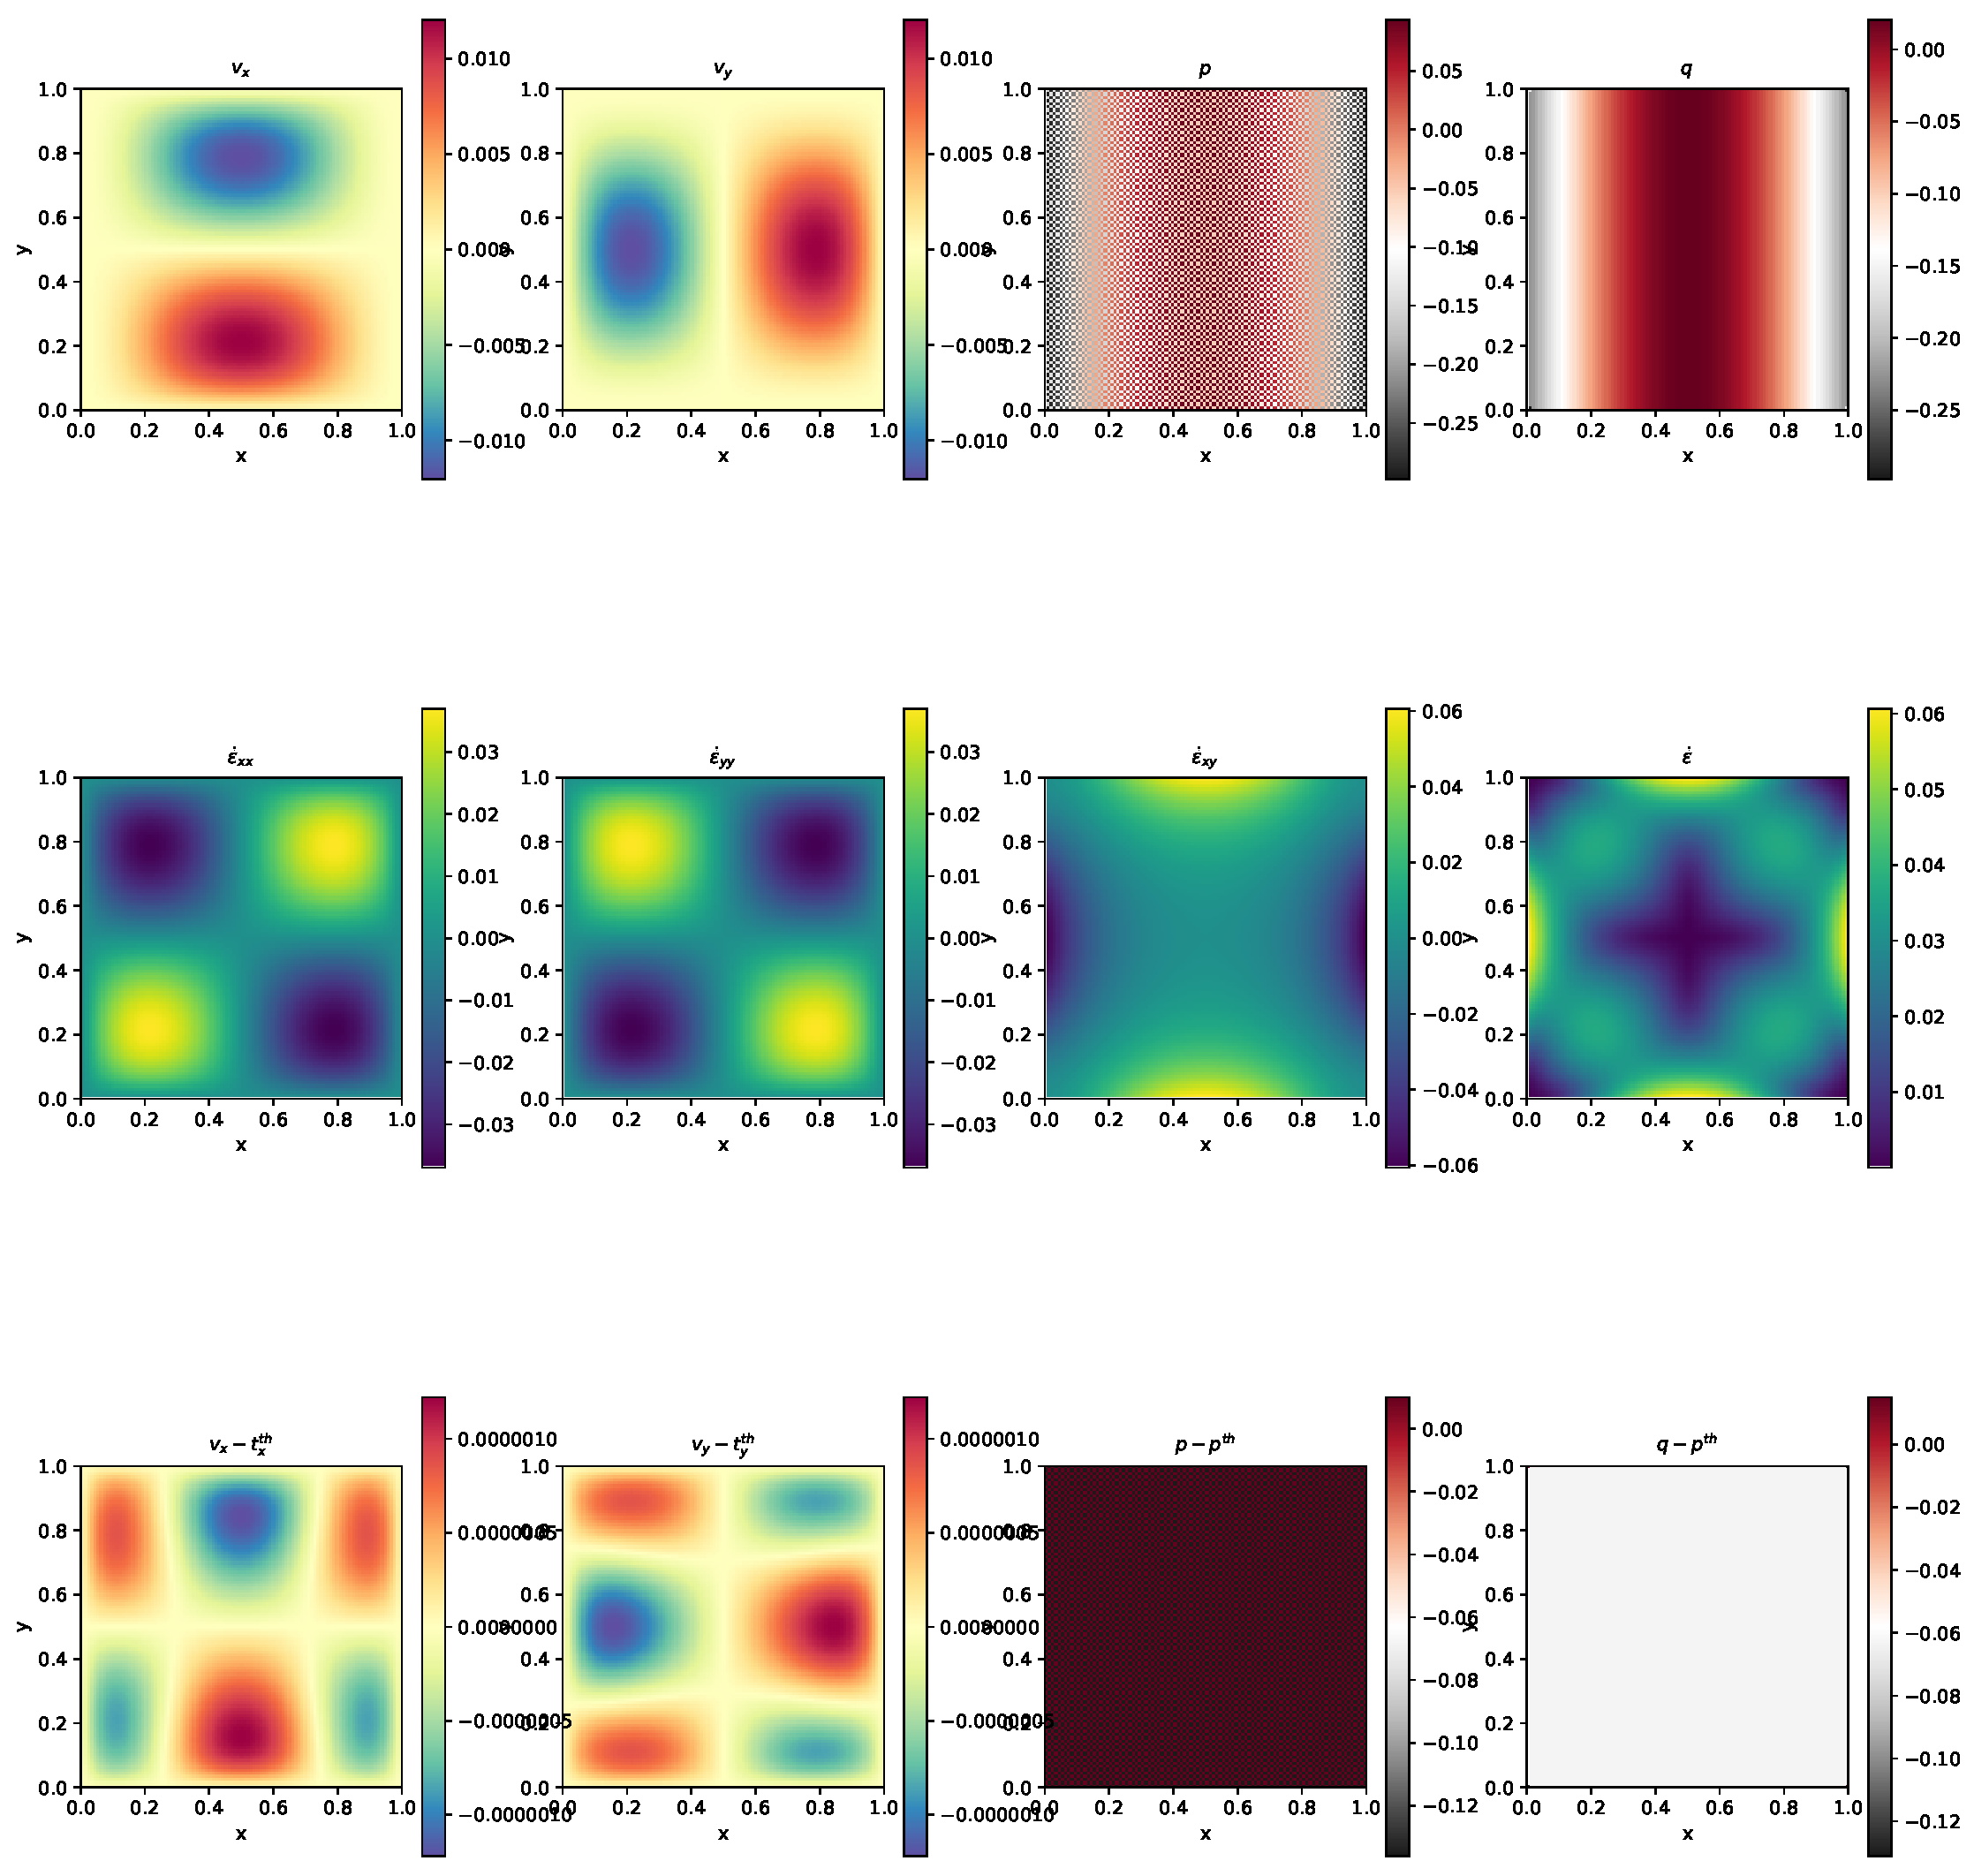
\includegraphics[width=16cm]{python_codes/fieldstone_saddlepoint/solution.pdf}


